\subsection{Classifying Global Extrema}
The theorems that we saw previously allowed us to classify \textbf{local extrema}. We want to identify \textbf{global extrema}.
\begin{center}
    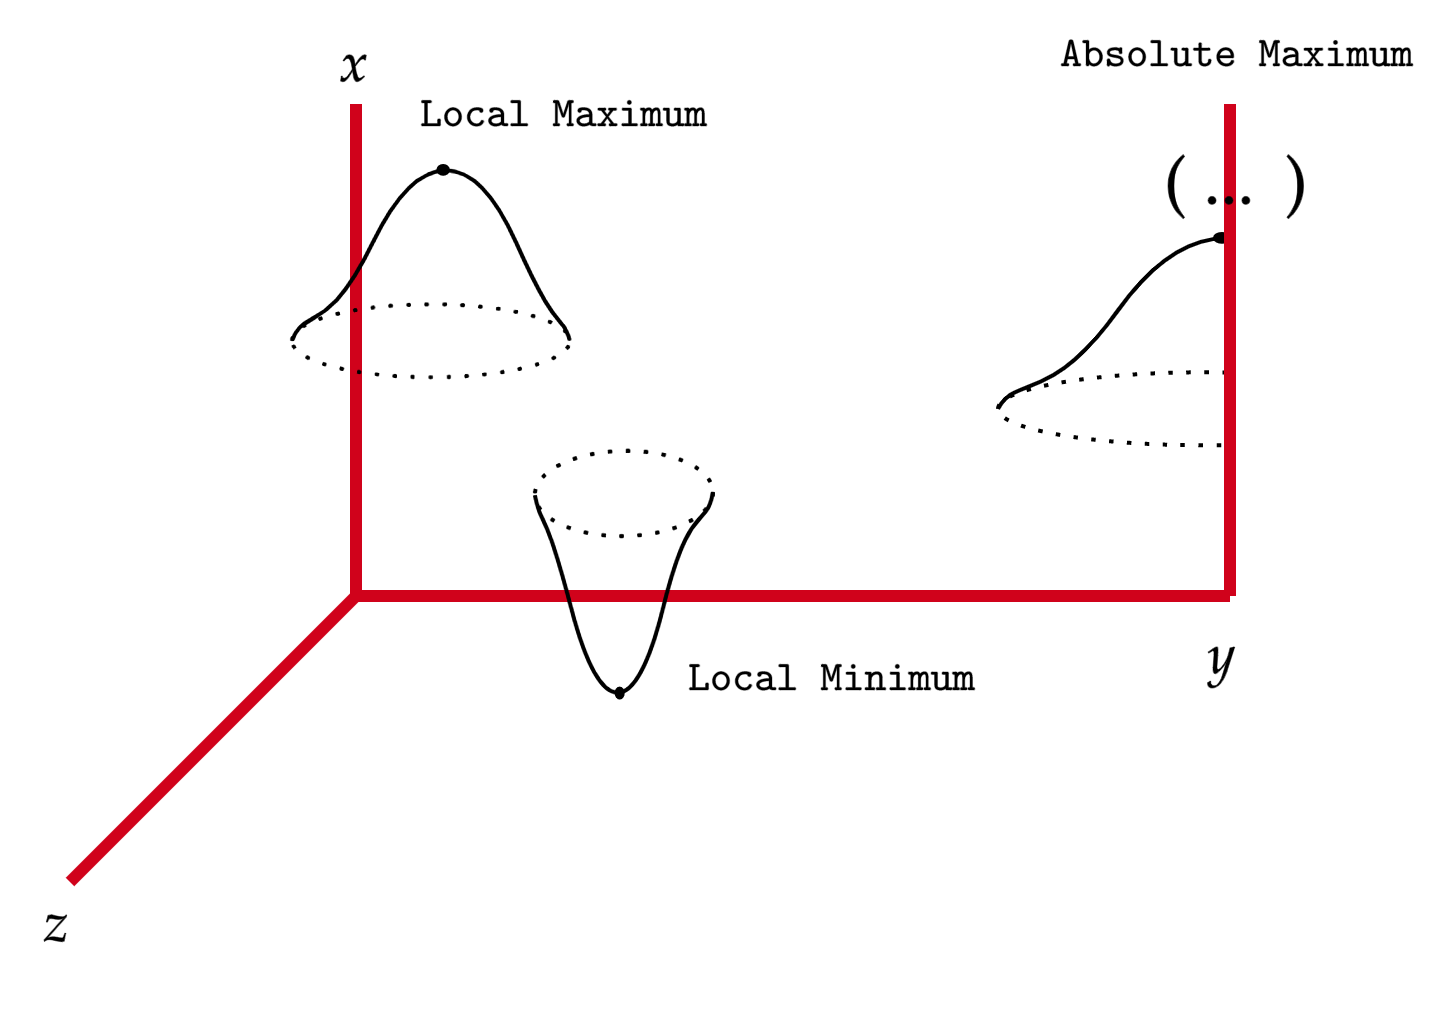
\includegraphics[width=0.7\linewidth]{figures/wk-4/fig-48.png}
\end{center}

\begin{defn}[Global Extrema]
    Let $f: A \subseteq \R^n \rightarrow \R$. $\mathbf{x}_0 \in A$ is a,
    \[
    \begin{cases}
        \text{Global Maximum} & \text{ if } f(\mathbf{x}) \leq f(\mathbf{x}_0)  \text{ for all } \mathbf{x} \in A \\
        \text{Global Minimum} & \text{ if } f(\mathbf{x}) \geq f(\mathbf{x}_0) \text{ for all } \mathbf{x} \in A
    \end{cases}
    \]
    
\end{defn}

\begin{marginfigure}
    A set $D \in \R^n$ is \textbf{bounded} if there is a number $M > 0$ such that $\|x\| < M$ for all $x \in D$. It is \textbf{closed} if it contains all of its boundary points. For example, the level sets of a continuous function are always closed.
\end{marginfigure}

\begin{defn}[Compact]
    A set is \textbf{compact} if it is closed and bounded.
\end{defn}

\begin{ex}{Compact Sets}{label}
    The following two sets are compact,
    \begin{enumerate}
        \item $\{(x,y) \mid x^2+y^2 \leq a^2\}$
        \item $\{(x,y) \mid a \leq |x| \leq b\}$
    \end{enumerate}
\end{ex}

\begin{thm}
 If $D \subseteq \R^n$ is compact, then $f: D \subseteq \R^n \rightarrow \R$ admits a global maximum and minimum, reached at some points of $D$.
\end{thm}

\begin{ex}{Finding Global Maxima and Minima}{label}
    Let $f: D \subseteq \R^2 \rightarrow \R$ be a continuous function defined on a compact set $D$. To find the global maximum and minimum,
    \begin{enumerate}
        \item Locate all critical points of $f$ in $\text{int}(D)$
        \item Locate all critical points of $f$ on $\partial D$
        \item Compute the value of $f$ on each critical point
        \item Compare these values to determine the largest and smallest
    \end{enumerate}
\end{ex}

\begin{ex}{Finding Global Maxima and Minima}{label}
    We want to find the absolute maximum and minimum of,
    \[f: A \subseteq \R^2 \rightarrow \R \text{ defined by } f(x,y) = x^2 + xy + y^2\]
    on the set $A = \{(x,y) \mid x^2+y^2 \leq 1\}$. We have that,
    \[\partial A = \{(x,y) \mid x^2+y^2 = 1\}\]
    Let $x := \cos \theta$ and $y := \sin \theta$ for $0 \leq \theta < 2 \pi$. Then,
    \begin{align*}
        \left. f\right|_{\partial A} = f(\cos \theta, \sin \theta) &= 1 + \cos \theta \sin \theta \\
        &= 1 + \frac{1}{2} \sin (2 \theta) =: g(\theta)
    \end{align*}
    Differentiating $g(\theta)$ gives that,
    \[g^{\prime}(\theta) = \cos (2 \theta) \implies \theta = \frac{\pi}{4}, \frac{3\pi}{4}\]
    This gives two points,
    \begin{align*}
        &f(\mathbf{p}_0) = f(0,0) = 0 \\
        &f\left(\mathbf{p}_1\right)=f\left(\cos \left(\frac{\pi}{4}\right), \sin \left(\frac{\pi}{4}\right)\right)=\frac{3}{2} = \frac{3}{2} \\
        &f\left(\mathbf{p}_1\right)=f\left(\cos \left(\frac{3\pi}{4}\right), \sin \left(\frac{3\pi}{4}\right)\right)=\frac{3}{2} = f\left(-\frac{\sqrt{2}}{2}, \frac{\sqrt{2}}{2}\right) = \frac{1}{2}
    \end{align*}
    There is a global minimum at $\mathbf{p}_0$ and a global maximum at $\mathbf{p}_1$.
\end{ex}

\begin{ex}{Finding Global Maxima and Minima}{label}
  We want to find the absolute maximum and minimum of,
    \[f: A \subseteq \R^2 \rightarrow \R \text{ defined by } f(x,y) = \sin x + \cos x\]
    on the set $A = \{(x,y) \mid x \in [0,2\pi] \text{ and } y \in [0,2\pi]\}$. Write,
    \[\partial A = \gamma_1 \cup \gamma_2 \cup \gamma_3 \cup \gamma_4\]
    If we consider the restriction,
    \[\left. f\right|_{\gamma_1} = f(x,0) = \sin x + 1 := g_1(x)\]
    on $x \in (0,2\pi)$, then we obtain that,
    \[g^{\prime}(x)=\cos x \implies x=\pi / 2 \text{ and. }x = 3 \pi / 2\]
    so the critical points are $(\pi / 2,0)$ and $(3 \pi / 2, 0)$. We can repeat this for each $\gamma_i$ to find the global maximum and minimum.
\end{ex}

\subsection{Constrained Extrema and Lagrange Multipliers}
We want to find the local extrema of a function $f$ restricted to a level set $g(\mathbf{x}_0) = c$. We call this a \textbf{constrained} extremum. 
\begin{thm}
    Suppose that $f: U \subseteq \R^n \rightarrow \R$ and $g: U \subseteq \R^n \rightarrow \R$ are of the class $C^1$. $f$ has a constrained extremum at $g(\mathbf{x}_0) = c$ if,
     \[(\mathbf{\nabla} f) (\mathbf{x}_0) = \lambda (\mathbf{\nabla} g)(\mathbf{x}_0)\]
     where $\lambda \in \R$ s called a \textbf{Lagrange multiplier}.
\end{thm}

\begin{rmk}
    The point $\mathbf{x}_0$ is a \textbf{critical point} of $f|U$. If $f|U$ has a maximum or minimum at $\mathbf{x}_0$, then $(\nabla f)(\mathbf{x}_0)$ is perpendicular to $U$ at $\mathbf{x}_0$.
\end{rmk}

\begin{rmk}
    $\lambda$ is an additional variable in the auxiliary function,
    \[L(x_1, \cdots, x_n, \lambda) = f(x_1, \cdots, x_n) - \lambda \cdot (g(x_1, \cdots, x_n) - c)\]
    To find the extreme points of $f | S$ we find the critical points of $L$,
    \begin{align*}
        &0 = h_{x_1} = f_{x_1} - \lambda g_{x_1} \\
        &\vdots \\
        &0 = h_{x_n} = f_{x_n} - \lambda g_{x_n} \\
        &0 = h_{\lambda} = g(x_1, \cdots, x_n) - c
    \end{align*}
\end{rmk}

\begin{ex}{Constrained Extrema}{label}
  Consider the function $f: \R^3 \rightarrow \R$ defined by,
  \[f(x,y,z) = xy + z^2\]
  on the sphere $x^2 + y^2 + z^2 = 1$. Define the Lagrange function $L := f+\lambda g=x y+z^2+\lambda\left(x^2+y^2+z^2\right)$. Now,
  \[
  \mathbf{\nabla} L=0 \implies \left\{\begin{array}{l}
    y+2 \lambda x=0 \\
    x+2 \lambda y=0 \\
    2 z+2 \lambda z=0 \\
    x^2+y^2+z^2=0
    \end{array}\right.
  \]
  We can then solve the system.
\end{ex}

\begin{ex}{Applications of Lagrange Multipliers}{label}
    We want to find the points on the curve
    \[g(x, y) = 17x^2+12xy + 8y^2 = 100\]
    which are closest to and farthest from the origin $(0,0)$. To do this, define the squared distance function $f(x, y) = x^2+y^2$.
\end{ex}

\begin{rmk}
    Given $k$ constraints,
    \[g_1(\mathbf{x})=c_1, \ldots, g_k(\mathbf{x})=c_k\]
    We have that $\left(\mathbf{\nabla} f\right)\left(\mathbf{x}_0\right)=\lambda_1\left(\mathbf{\nabla} g_0\right)\left(\mathbf{x}_0\right)+\ldots+\lambda_k\left(\mathbf{\nabla} g_k \right)\left(\mathbf{x}_0\right)$.
\end{rmk}